In the last chapter we saw that the \gls{shg} intensity in a given crystal is related to the point group, order parameter, band structure, etc. of that crystal via the susceptibility tensor $\chi_{ijk}$.
It is also obvious from \cref{sec:neumann} that the ideal scenario is to be able to measure as many of the numbers $\chi_{ijk}$ as possible; after all, if you only measured the $xx$ component of \cref{eq:c2eps,eq:d3deps}, you would have obtained essentially no information about your crystal whatsoever.
The \gls{shg} setup that we built (whose design is mostly credited to Torchinsky and Hsieh\citep{torchinsky_low_2014}, with some improvements by us which I will discuss below) was designed with exactly this goal in mind.
There are two key insights which make this design work: one, the light is obliquely incident on the sample so there is some component of $\bm{E}^\mathrm{in}$ directed along the sample normal, and two, we rotate the plane of incidence so that the in-plane field direction sweeps an entire $360^\circ$.
The first point allows us to measure elements of $\chi_{ijk}$ with $z$ indices\footnote{Here and unless otherwise noted I define the sample normal to be the $z$ axis.}, and the second point makes sure we get all of the $x$ and $y$ elements of $\chi_{ijk}$ too.
All of the tensor elements are thus given a chance to contribute to the \gls{shg} intensity in a given experiment.

With those considerations in mind, let me proceed to give a schematic description of our \gls{shg} setup.
Some of the choices we made may seem arbitrary right now, but I will go over them in detail in \cref{sec:beforeyoubuild}.
The starting point is our regenerative amplifier (Spectra-Physics Spitfire Sptf-100f-5k-xp), which produces $100$ \si{fs} $800$ \si{nm} pulses at a $5$ \si{kHz} repetition rate from an $86$ \si{MHz} seed laser (Spectra-Physics Tsunami 3941-M1S). 
$90\%$ of the beam is split off to power an \gls{opa}, and the remaining $10\%$ is used for the \gls{shg} probe beam.
After passing through an optical telescope, which creates a collimated beam of width $1-2$ \si{mm}, this beam is attenuated with a polarizer - half-wave plate - polarizer triplet, and then elliptically polarized with a quarter-wave plate and half-wave plate in series.
The ellipticity at this stage is set so the light is perfectly circularly polarized following transmission through a phase mask, as described below.

After passing through these polarization optics, the beam is focused with a lens onto the aforementioned phase mask, which acts as a transmissive diffraction grating and separates the beam into multiple different diffraction orders.
The $+1$ order diffraction comes off at an angle of roughly $7^\circ$, while the other orders are blocked with anodized aluminum foil. 
This (diverging) beam then propogates at $7^\circ$ to the optical axis before meeting a lens set at the appropriate distance so as to both collimate the beam and rectify the $7^\circ$ progation angle.
Then, the light passes through a dichroic mirror (which transmits $800$ \si{nm} and reflects $400$ \si{nm}), becomes linearly polarized by a wire-grid polarizer, and is then focused onto the sample at a $10^\circ$ angle of incidence by passing through the edge of a $1$ \si{in}-diameter $50$ \si{mm} achromatic focusing lens.
The interaction between the light and the sample causes \gls{shg} to be radiated in reflection at the same $10^\circ$ angle of incidence, so that the \gls{shg} beam passes through the opposite side of the $50$ \si{mm} lens before passing through a second, independent polarizer which is used to control the polarization of the measured light.

\begin{figure}
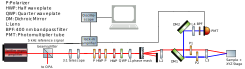
\includegraphics[width=\textwidth]{gfx/ch3/pdf/setup.pdf}
\caption{\label{fig:setup}Schematic drawing of the \gls{shg} setup used in this research. After \citet{morey_automated_2024}.}
\end{figure}

Finally, the polarized output reflects off of two dichroic mirrors (oriented in such a way as to cancel the differing effect of the Fresnel equations on the reflectivity of S and P polarized light) and is focused through a $400$ \si{nm} bandpass filter onto a \gls{pmt} by a $400$ \si{mm} lens.
The current output of the \gls{pmt} is filtered by a lock-in amplifier (for static \gls{shg}, set to the $5$ \si{kHz} repetition rate of the laser) and read out on an oscilloscope.
The phase mask, incoming polarizer, and outgoing polarizer are mounted on rotating lens tubes which are connected via pulley to a common motor shaft driven by a brushless DC motor.
The motor thus continuously rotates the plane of incidence of the experiment, since the latter is entirely defined by the phase mask and the polarizers.
The rotation angle is tracked as a function of time by an optical rotary encoder, consisting of a laser pointer passed through a chopper wheel (with 100 slots) mounted at the end of the motor shaft and detected via photodiode.
The encoder signal and the lock-in signal are both sent to a homemade oscilloscope (an Arduino Uno microcontroller which separates the lock-in signal into different individual rotations by looking for peaks in the encoder signal), the output of which is sent to a computer for further data processing.

\section{Before you build}\label{sec:beforeyoubuild}

I list here a few essential aspects of \gls{shg} that should be considered before designing a new setup.

\subsection{Spot size}

One of the most important quantities in an \gls{shg} setup is the diameter of the probe spot.
Ideally, this diameter is as small as possible, so as to measure the smallest samples or domain sizes.
However, there is an important caveat: for constant fluence (i.e. supposing we are limited by the sample damage threshold), the \gls{shg} signal to noise ratio scales linearly in the area excited by the probe, and thus \gls{shg} microscopes have a difficult time measuring small \gls{shg} signals compared to traditional \gls{shg} setups with a larger excitation area.
To see this, let us say that our detector measures the number of photons per \gls{shg} pulse, which is proportional to the pulse energy $U_p(2\omega)$.
Assuming the input and output pulse intensity profiles have the shape of a square wave with width $\tau$ and height $I_p(\omega)$ and $I_p(2\omega)$, respectively, we have
\begin{equation}
U_p(2\omega) = A I_p(2\omega) \tau
\end{equation}
and
\begin{equation}
U_p(\omega) = A I_p(\omega) \tau
\end{equation}
where $A$ is the area of the beam at the sample surface.
The \gls{shg} intensity is proportional to the square of the input intensity
\begin{equation}
I_p(2\omega) \propto I_p^2(\omega)
\end{equation}
so that
\begin{equation}
U_p(2\omega) \propto \frac{U_p^2(\omega)}{A\tau}.
\end{equation}
Substituting for the fluence $f$
\begin{equation}
f(\omega) = \frac{U_p(\omega)}{A}
\end{equation}
we have
\begin{equation}
U_p(2\omega) \propto \frac{f^2(\omega)A}{\tau}
\end{equation}
i.e., if we hold the fluence constant at the sample damage threshold, the number of photons in the generated \gls{shg} pulse is proportional to the excitation area and inverse to the pulse width.
The signal to noise ratio is then given by
\begin{equation}
\mathrm{SNR} \propto \frac{U_p(2\omega)}{\sqrt{r}}
\end{equation}
where $r$ is the system repetition rate.

\subsection{Oblique vs. normal incidence}

While all of the results presented in this thesis utilized the setup in \cref{fig:setup}, where the incident beam makes a small angle with respect to the sample normal, plenty of groups use a different approach where that angle is set to $0^\circ$.
This has the obvious disadvantage of not specifying all of the tensor elements, since any element $\chi_{ijk}$ with $i, j, k = z$ is not accessible in this geometry.
However, in some cases this can actually be something of an advantage.
For example, sometimes unwanted \gls{shg} contributions (see \cref{sec:manyshgterms}) may be avoided in the normal incidence geometry, assuming the \gls{na} of the focusing optic is small enough that longitudinal components of the electric field are nearly zero.
Furthermore, in some materials the order parameter only couples to one or two elements of $\chi_{ijk}$; if none of these elements have a $z$ index, it is needless to complicate the analysis with oblique incidence.

In my experience, oblique incidence seems to be useful in two broad cases.
For one thing, some order parameters only show up in the $z$ components of $\chi_{ijk}$ (this is the case in \tastwo, see \cref{sec:tastwo}), in which case one obviously needs a nonzero angle of incidence to access these components.
A more subtle point is that, even if in practice all of the phenomenology of a particular sample only shows up in the $x$ and $y$ indices of $\chi_{ijk}$, still one must measure the full tensor to \emph{rule out} unseen phenomenology in the other indices.
Both the \ce{CaMn2Bi2} (\cref{ch:ch5}) and \ce{CuBr2} (\cref{ch:ch6}) works presented in this thesis are examples of exactly this point, where the main scientific arguments involve either comparing \gls{shg} patterns in two domains or comparing oscillation amplitudes in different polarization channels.
Clearly one needs to know all of the tensor elements to make those arguments exact.
